\newcommand{\IncludeSchoolTemplate}[2]{
	\vspace*{-7em}
	\makebox[\textwidth]{
		\begin{tikzpicture}[
			every node/.style={anchor=north west,inner sep=0pt},
			x=1mm, y=1mm]
			\node (templatepage) at (0,0)
			{\includegraphics[width=\paperwidth,page=#1]{./summary.pdf}};
			#2
		\end{tikzpicture}
	}
	\newpage
}

\pagenumbering{gobble}

\selectlanguage{german}

\includegraphics[width=\textwidth]{./grafiken/school-header.png}
{\centering
	\vskip1cm
	Fachrichtung Informatik
	\vskip2cm
	Schuljahr 2020/21
	\vskip4cm
	\Huge\textbf{ERM}
	\vskip10pt
	\large
	Gesamtprojekt
	\vskip5pt
	\Huge\textbf{Endkundenportal: Registrierung und Maschinenpark}
	\small
	\vskip4cm
	\begin{flushleft}
		\textbf{Ausgeführt von:}\tabto{9cm}\textbf{Betreuer/Beteuerin:}\linebreak
		\ThRealAuthorNameOne, \ThAuthorsClass-\ThAuthorOneNumber\tabto{9cm}\ThSupervisorName\linebreak
		\ThRealAuthorNameTwo, \ThAuthorsClass-\ThAuthorTwoNumber
		\vskip1cm
		\ThPhysicalLocation, am \today
		\vskip1cm
		\hrule
		Abgabevermerk:\linebreak
		Datum:\tabto{10cm}Betreuer/Beteuerin:
	\end{flushleft}
}



\selectlanguage{german}
\chapter*{\hspace{5pt}Erklärung gemäß Prüfungsordnung}
„Ich erkläre an Eides statt, dass ich die vorliegende Diplomarbeit selbstständig und ohne fremde Hilfe verfasst, andere als die angegebenen Quellen und Hilfsmittel nicht benutzt und alle den benutzten Quellen wörtlich oder sinngemäß entnommenen Stellen als solche kenntlich gemacht habe.“

\ThPhysicalLocation, \today\tabto{9cm}{Verfasser*innen:}
\selectlanguage{english}

\SignatureLine{\ThRealAuthorNameOne}
\SignatureLine{\ThRealAuthorNameTwo}
\newpage
\IncludeSchoolTemplate{1}{
	\node at (77,-28)
		{Informatik};
	\node at (77,-63)
		{\ThRealAuthorNameOne};
	\node at (77,-70)
		{\ThRealAuthorNameTwo};
	\node at (77,-80)
		{2020/21};
	\node at (77,-92)
		{Endkundenportal: Registrierung und Maschinenpark};
	\node at (77,-109)
		{\ThPartnerName};
	\node at (77,-127) [text width=305,align=justify] {
		\fontsize{12pt}{12pt}
		\selectfont
		\par
		Ziel des Projekts war die Entwicklung einer Plattform mit einer i18n und dynamischen Registrierungsmöglichkeit. Kunden können in Zukunft ihre eigenen Maschinen im Endkundenportal hinzufügen. Auch soll es im Endkundenportal verschiedene Benutzergruppen mit dementsprechenden Rechten geben. Das Portal soll verschiedene Funktionen und Berechtigungen darstellen.
		%Im Rahmen der Matura besteht die Aufgabe von ERM darin, eine länderspezifische Registrierung mit jeweiliger Validierung für die Endkunden auf der ganzen Welt bereitzustellen und dieser Prozess soll so einfach und schnell wie möglich für den Benutzer sein. Nach der Registrierung soll jeder registrierte Benutzer einen Maschinenpark anlegen können, wo dieser sich seine eigenen Maschinen speichern kann und somit schnell zu näheren Infos zu diesem Gerät, wie zum Beispiel Highlights, Technische Daten oder Betriebsanleitung, gelangt.
		%\vskip10pt
		%Das Backend soll in C\# mit .NET CORE 3.1 und das Frontend mit Angular in TypeScript realisiert werden.
		\par
		
	};
	\node at (77,-174) [text width=300,align=justify] {
		\fontsize{12pt}{12pt}
		\selectfont
		\par
		Das Registrierungsformular wird im Frontend je nach Länder- und Sprachenwahl dynamisch aufgebaut. Die Auswahl, Anordnung und Validierung variiert je nach Land. Bei erfolgreicher Registrierung über Auth0 wird der User im Backend gespeichert und ihm stehen weitere Features zur Verfügung. Die Usereingaben werden im Frontend und im Backend validiert um jegliche Fehler zu vermeiden. Die weiteren Aufrufe sind mit JWT-Tokens gesichert.
		\vskip10pt
		\par
	};
	\node at (77, -222) [text width=300,align=justify] {
		\fontsize{12pt}{12pt}
		\selectfont
		\par
		Das Ergebnis ist ein Endkundenportal, was den User ermöglich, seine Maschinen zu speichern und immer schnell alle wichtigen Informationen darüber herauszufinden. Die Registrierung ist länderspezifisch. Weiters hat \ThPartnerName \ eine direkte Endkundenverbindung, die es zuvor nicht gab. Dazu wurde das Backend für ein FAQ-Bereich erstellt. Dabei werden die gestellten fragen nach dem beantworten automatisch in 15 Sprachen übersetzt und gespeichert.
	};
}
\IncludeSchoolTemplate{2}{
	\node at (77,-28)
		{Informatik};
	\node at (77,-80){
		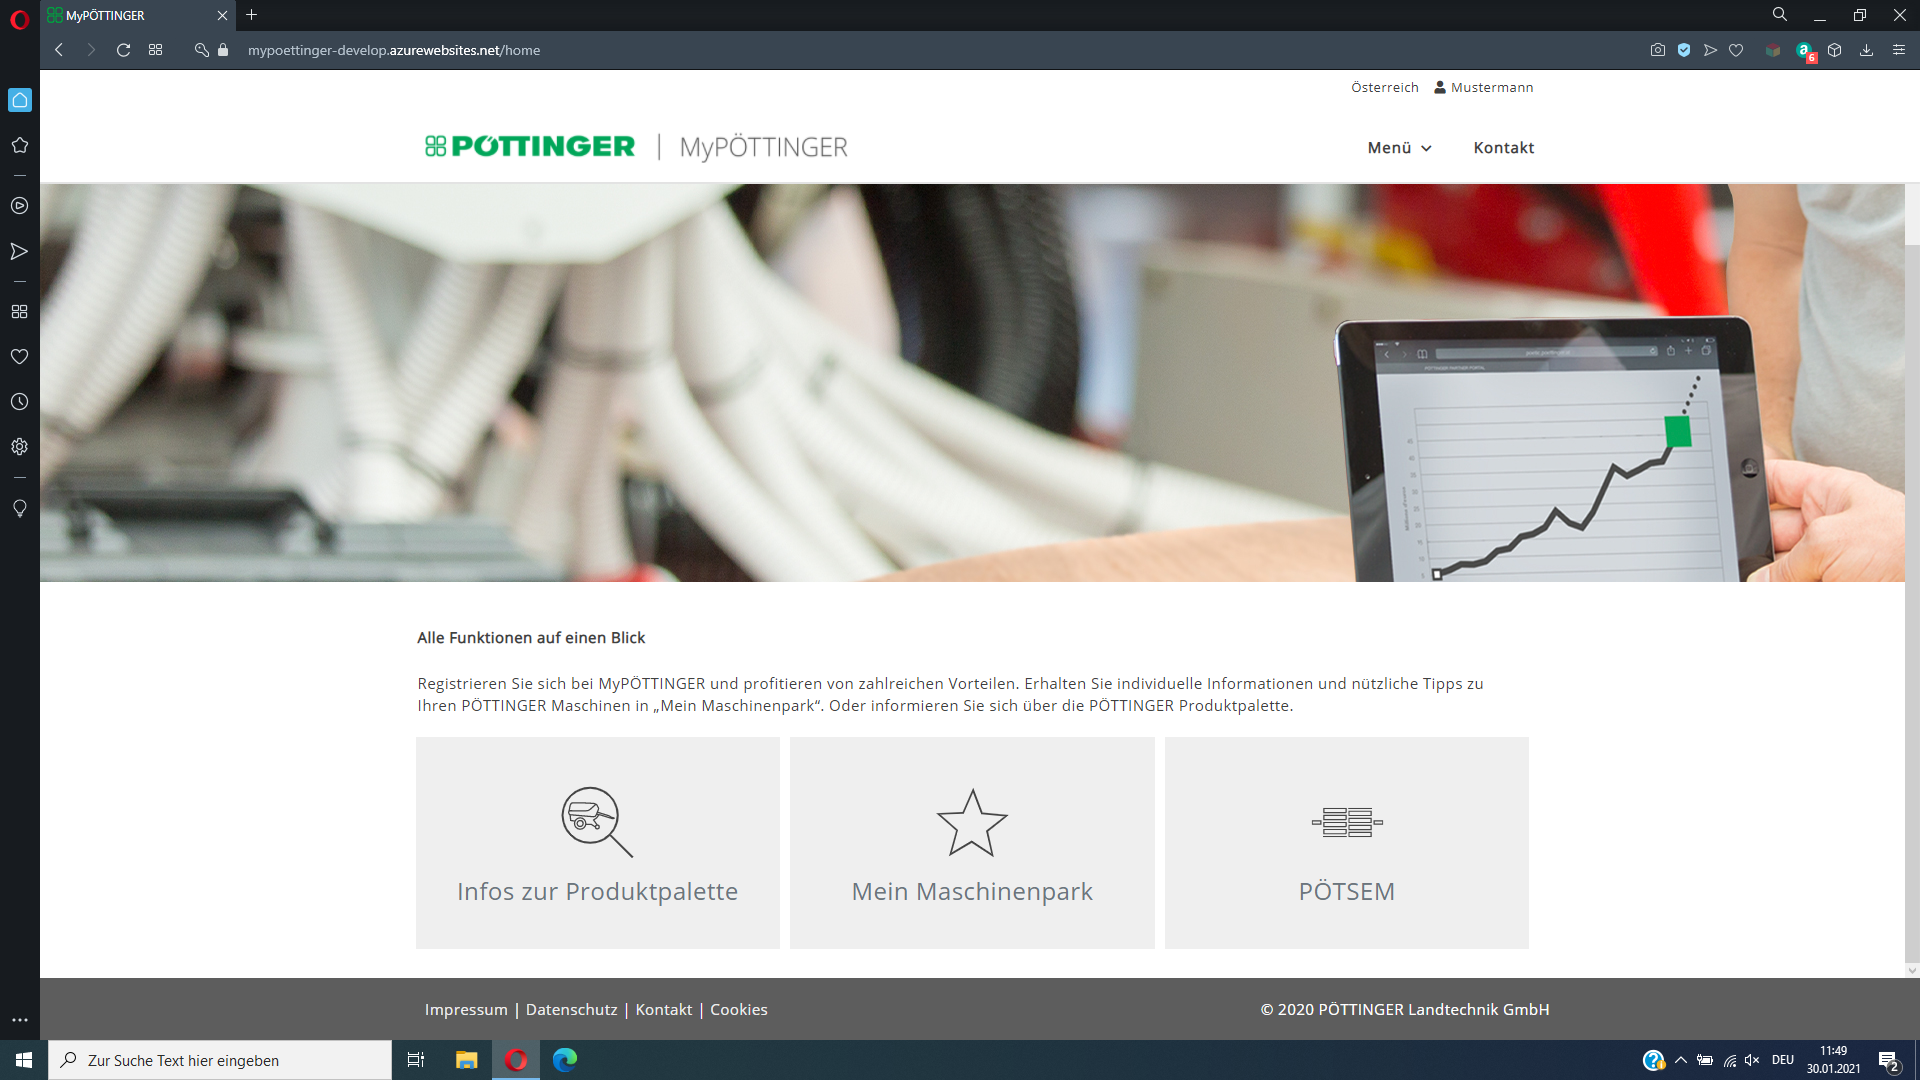
\includegraphics[width=310pt,trim=0pt 0pt 0pt 0pt,clip]{./grafiken/erm_home_logged_in.png}
	};
	\node at (77,-171) [text width=305]
		{Auf diesem Screenshot sieht man die Hauptseite als eingeloggter Benutzer, von wo man alles erreichen kann.};
	\node at (77,-220)
		{--};
	\node at (77,-239)
		{Öffentlich; Bibliothek der \ThSchoolName};
}
\IncludeSchoolTemplate{3}{
	\node at (76,-28)
		{Informatics};
	\node at (77,-63)
		{\ThRealAuthorNameOne};
	\node at (77,-70)
		{\ThRealAuthorNameTwo};
	\node at (77,-80)
		{2020/21};
	\node at (77,-92)
		{Sample Project};
	\node at (77,-109)
		{\ThPartnerName};
	\node at (77,-125) [text width=305,align=justify] {
		\fontsize{12pt}{12pt}
		\selectfont
		\par
		Ziel des Projekts war die Entwicklung einer Plattform mit einer i18n und dynamischen Registrierungsmöglichkeit. Kunden können in Zukunft ihre eigenen Maschinen im Endkundenportal hinzufügen. Auch soll es im Endkundenportal verschiedene Benutzergruppen mit dementsprechenden Rechten geben. Das Portal soll verschiedene Funktionen und Berechtigungen darstellen.
		%Im Rahmen der Matura besteht die Aufgabe von ERM darin, eine länderspezifische Registrierung mit jeweiliger Validierung für die Endkunden auf der ganzen Welt bereitzustellen und dieser Prozess soll so einfach und schnell wie möglich für den Benutzer sein. Nach der Registrierung soll jeder registrierte Benutzer einen Maschinenpark anlegen können, wo dieser sich seine eigenen Maschinen speichern kann und somit schnell zu näheren Infos zu diesem Gerät, wie zum Beispiel Highlights, Technische Daten oder Betriebsanleitung, gelangt.
		%\vskip10pt
		\par
		Das Backend soll in C\# und das Frontend in TypeScript realisiert werden.
	};
	\node at (77,-173) [text width=300,align=justify] {
		\fontsize{12pt}{12pt}
		\selectfont
		\par
		Das Registrierungsformular wird im Frontend je nach Länder- und Sprachenwahl dynamisch aufgebaut. Die Auswahl, Anordnung und Validierung variiert je nach Land. Bei erfolgreicher Registrierung über Auth0 wird der User im Backend gespeichert und ihm stehen weitere Features zuverfügung. Die Usereingaben werden im Frontend und im Backend validiert um jegliche Fehler zu vermeiden. Die weiteren Aufrufe sind mit JWT-Tokens gesichert.
		\vskip10pt
		\par
	};
	\node at (77, -225) [text width=300,align=justify] {
		\fontsize{12pt}{12pt}
		\selectfont
		\par
		Das Ergebnis ist ein Endkundenportal, was den User ermöglich, seine Maschinen zu speichern und immer schnell alle wichtigen Informationen darüber herauszufinden. Weiters hat \ThPartnerName \ eine direkte Endkundenverbindung, die es zuvor nicht gab.
	};
}
\IncludeSchoolTemplate{4}{
	\node at (76,-28)
		{Informatics};
	\node at (77,-75){
		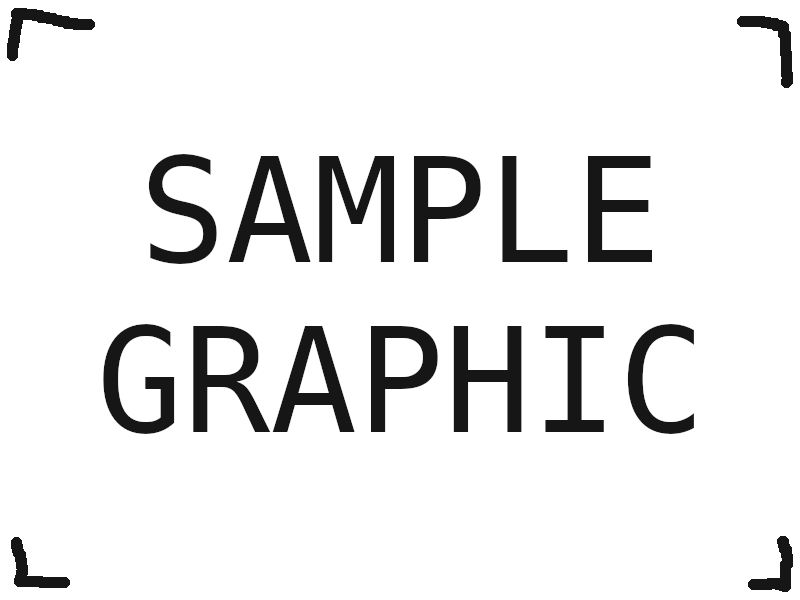
\includegraphics[width=310pt,trim=0pt 0pt 0pt 0pt,clip]{./grafiken/sample_graphic.png}
	};
	\node at (77,-166) [text width=305,align=center]
		{\emph{Screenshot of the program}};
	\node at (77,-220)
		{--};
	\node at (77,-240)
		{Public; Library of the \ThSchoolName};
}